
\section{Benchmark}
\label{sec:bench}
In this section, we show the results of the benchmarks that we performed to assess the performance of our implementations in various settings. We also discuss the implications of the results that we found.
\subsection{Setup}
We ran the benchmark on PostgreSQL 9.1.9 and MADlib v3.0 on a single machine on a gigabit Ethernet cluster which runs Ubuntu 12.04 LTS and has 4GB RAM, a 10GB SATA HDD and a Core 2 Duo 2.4GHz CPU. 

To benchmark the performance of GP for Symbolic Regression we used a synthetic dataset containing 100,000 rows, 3 inputs and 1 output. The function we used to generate the data is $x_1*(x_2^2+x_3)$.

To benchmark the performance of AdaBoost, we used BUPA liver disorder dataset which contains blood test results of 345 male individuals. This dataset is available at \url{http://www.cs.huji.ac.il/~shais/datasets/ClassificationDatasets.html}. We also used a synthetic dataset which consisted of $240000\times11$ matrix where first 10 columns are real valued random numbers and the last column indicates the class.

Each run of our algorithms inside MADlib was cold start meaning that we cleared the caches and restarted the database service (PostgreSQL) for every run.
\subsection{Results}
Tables~\ref{tab:gp}, \ref{tab:adaBupa1}, \ref{tab:adaBupa2}, \ref{tab:adaSynth1} and \ref{tab:adaSynth2} summarize our benchmark results. Table~\ref{tab:gp} shows <Filled by Franck>. In Table~\ref{tab:adaBupa1}, we record the runtimes of row-by-row execution, batched execution and all-in-memory execution of AdaBoost inside MADlib. In Table~\ref{tab:adaBupa2}, we record the runtimes of the same algorithm when it reads data from a file or from PostgreSQL database outside MADlib or loads data into memory from Postgres residing inside MADlib. In all cases we varied the number of iterations parameter. Table~\ref{tab:adaSynth1} shows the runtimes and Table~\ref{tab:adaSynth2} shows the memory usage of row-by-row execution, batched execution and all-in-memory execution of AdaBoost when it is run on a synthetic dataset of varying size.   

\begin{table}[!htbp]
\centering
\begin{tabular}{lcc}
\end{tabular}
\caption{GP runtimes on synthetic dataset}
\label{tab:gp}
\end{table}

\begin{table}[!htbp]
\small
\centering
\begin{tabular}{|c|c|c|c|c|c|c|}
\hline
\multirow{2}{*}{NumIter} & \multicolumn{6}{|c|}{Runtimes (sec)}\\
\cline{2-7}
& All-in-Memory & 2 Batches & 5 Batches & 10 Batches & 50 Batches & Row-by-Row\\
\hline
50 &1.04 &96.72 &99.23 &149.96 &213.31 &314.75 \\
\hline
100 &2.09 &147.90 &236.93 &527.41 &770.55 &1215.30 \\
\hline
150 &2.69 &283.44 &548.98 &844.80 &1746.58 &2727.17 \\ 
\hline
200 &3.39 &675.45 &986.81 &1107.41 &3118.15 &4334.23 \\ 
\hline
250 &4.18 &1052.99 &1728.76 &2546.37 &3118.154 &6525.33 \\ 
\hline
300 &4.88 &1566.79 &2814.76 &3926.46 &6367.52 &9041.89 \\ 
\hline
350 &5.72 &2578.63 &3789.65 &5444.76 &8567.15 &11822.67 \\ 
\hline
400 &6.58 &4548.88 &5567.59 &9720.97 &12319.85 &16878.20 \\ 
\hline
450 &7.58 &7143.48 &8869.80 &12414.58 &17613.34 &24683.87 \\ 
\hline
500 &7.96 &9776.36 &11934.97 &16977.72 &23814.81 &30417.70 \\
\hline
\end{tabular}
\caption{AdaBoost runtimes on BUPA liver disorder dataset (Row-by-Row vs. Batched vs. All-in-Memory execution).}
\label{tab:adaBupa1}
\end{table}

\begin{table}[!htbp]
\small
\centering
\begin{tabular}{|c|c|c|c|}
\hline
\multirow{3}{*}{NumIter}&\multicolumn{3}{|c|}{Runtimes (sec)}\\
\cline{2-4}
&Outside MADlib&Outside MADlib&\multirow{2}{*}{Inside MADlib}\\
&from PostgreSQL&from File&\\
\hline
500&6.73 &6.37 &7.96 \\
\hline
1000&10.85 &12.23 &14.01 \\\hline
1500&16.82 &18.27 &20.43 \\\hline
2000&21.87 &24.56 &27.50 \\\hline
2500&27.13 &30.92 &33.52 \\\hline
3000&32.95 &38.25 &40.27 \\\hline
3500&38.11 &43.28 &47.11 \\\hline
4000&43.51 &50.45 &54.48 \\\hline
4500&50.86 &57.02 &60.51 \\\hline
5000&57.86 &62.97 &72.63 \\\hline
7000&82.00 &88.12 &133.256 \\\hline
10000&127.60 &124.88 &252.98 \\
\hline
\end{tabular}
\caption{AdaBoost runtimes on BUPA liver disorder dataset (Inside vs. Outside MADlib).}
\label{tab:adaBupa2}
\end{table}

\begin{table}[!htbp]
\small
\centering
\begin{tabular}{|c|c|c|c|c|c|c|}
\hline
\multirow{2}{*}{NumTuples} & \multicolumn{6}{|c|}{Runtimes (sec)}\\
\cline{2-7}
& All-in-Memory & 2 Batches & 5 Batches & 10 Batches & 50 Batches & Row-by-Row\\
\hline
20000&92.02 &10938.07 &11932.44 &12702.27 &14063.23 &19688.52 \\
\hline
30000&143.13 &14379.26 &15418.72 &16838.87 &18024.70 &25595.08 \\
\hline
40000&201.38 &17579.04 &19390.21 &20911.01 &22690.67 &31993.85 \\
\hline
50000&252.59 &23106.67 &25055.43 &26324.06 &29708.58 &41592.01 \\
\hline
60000&320.38 &29576.54 &32432.05 &34126.77 &38026.98 &53237.77 \\
\hline
\end{tabular}
\caption{AdaBoost runtimes on synthetic dataset.}
\label{tab:adaSynth1}
\end{table}

\begin{table}[!htbp]
\small
\centering
\begin{tabular}{|c|c|c|c|c|c|c|}
\hline
\multirow{2}{*}{NumTuples} & \multicolumn{6}{|c|}{Memory Usage (\%)}\\
\cline{2-7}
& All-in-Memory & 2 Batches & 5 Batches & 10 Batches & 50 Batches & Row-by-Row\\
\hline
80000& 9.0&7.8&4.1 &3.2 &2.7&2.6 \\
\hline
120000& 12.4&7.9 &4.2 &3.4&3.0 &2.7 \\
\hline
160000& 15.9&7.9 &4.2 &3.4 &3.2 &2.7 \\
\hline
200000& 18.1&8.0 &4.3 &3.6 &3.2 &2.6 \\
\hline
240000& 21.3&8.2 &4.4 &3.7 &3.4 &2.7 \\
\hline
\end{tabular}
\caption{AdaBoost memory usage for synthetic dataset}
\label{tab:adaSynth2}
\end{table}

As we can see from the tables, runtime of both of the algorithms increase as we increase the number of independent variables. Running the algorithms using MADlib takes more time than bypassing MADlib altogether when data can be fit into memory. Running the algorithms using MADlib is advantageous when the dataset cannot be fit into memory. Batched execution is more efficient in terms of run time than row by row execution in terms of run time. It is more efficient than reading the whole dataset into memory in terms of memory usage.

\subsection{Analysis}
\subsubsection*{\itshape Effect of varying independent variables on runtime.}

\subsubsection*{\itshape Performance inside and outside MADlib}
\begin{figure}[ht]
\centering
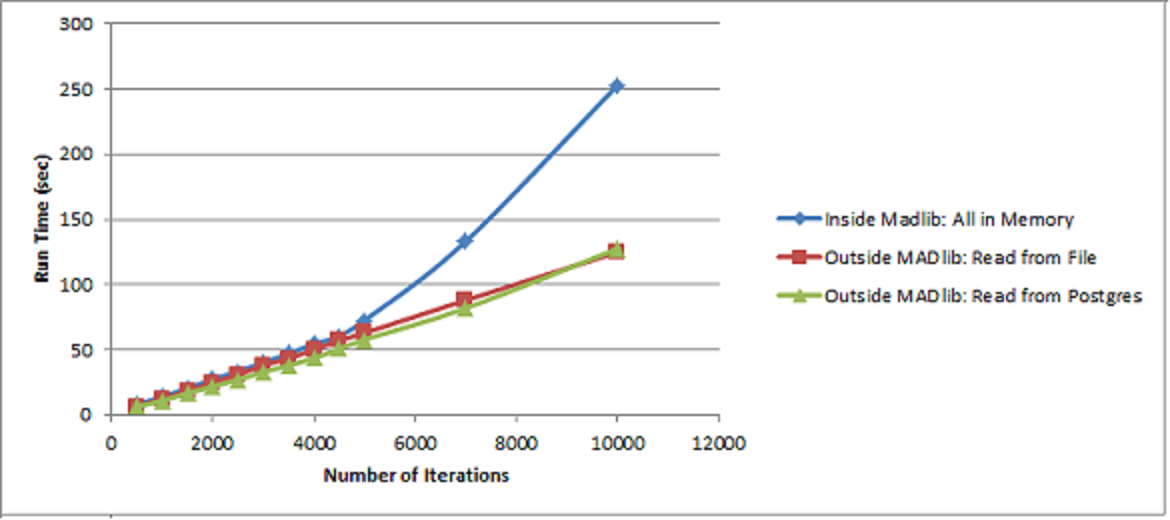
\includegraphics[width=0.8\textwidth]{ada1.png}
\caption{Runtimes of AdaBoost algorithm inside and outside MADlib.}
\label{fig:adainout}
\end{figure}

\subsubsection*{\itshape Performance of batched execution.}
\begin{figure}[ht]
\centering
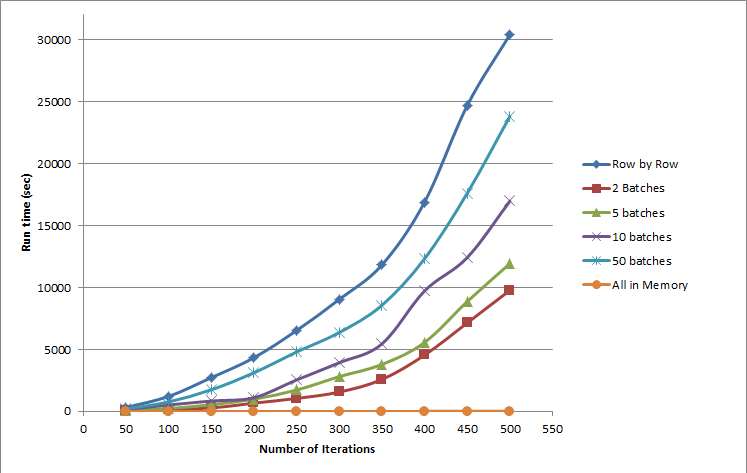
\includegraphics[width=0.8\textwidth]{ada2.png}
\caption{Runtimes of row-by-row, batched and all-in-memory execution of AdaBoost algorithm on BUPA liver disorder dataset.}
\label{fig:adabatch1}
\end{figure}

\begin{figure}[ht]
\centering
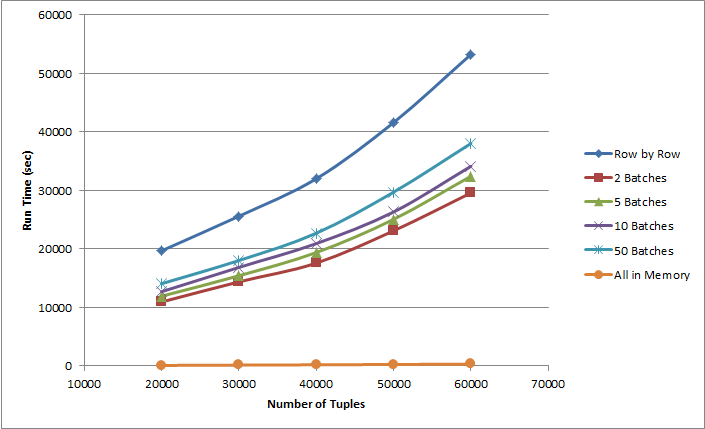
\includegraphics[width=0.8\textwidth]{ada3.png}
\caption{Runtimes of row-by-row, batched and all-in-memory execution of AdaBoost algorithm on synthetic dataset.}
\label{fig:adabatch2}
\end{figure}

\subsubsection*{\itshape Effect of varying independent variables on memory usage.}
\begin{figure}[ht]
\centering
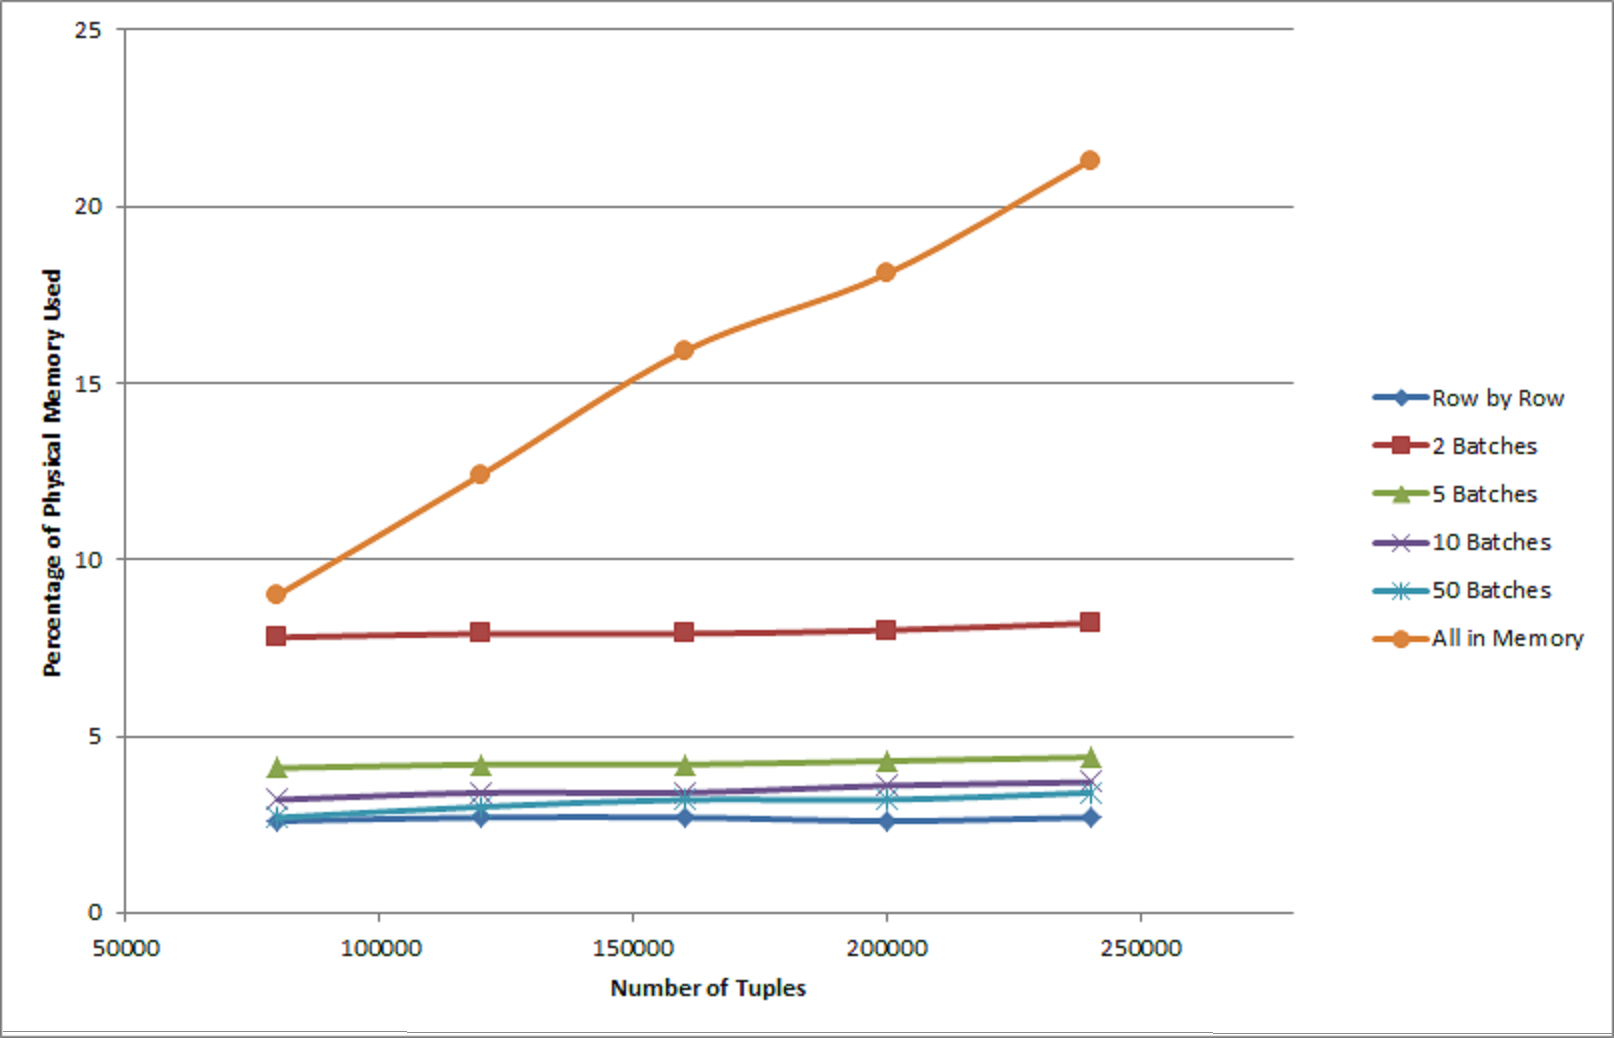
\includegraphics[width=0.8\textwidth]{ada4.png}
\caption{Memory usage by AdaBoost algorithm on synthetic dataset.}
\label{fig:adamem}
\end{figure}
